\documentclass{patmorin}
\usepackage[utf8]{inputenc}
\usepackage{amsthm,amsmath,graphicx}
\usepackage{array}
\usepackage{pat}
\usepackage{hyperref}
\usepackage[dvipsnames]{xcolor}
\definecolor{linkblue}{named}{Blue}
\hypersetup{colorlinks=true, linkcolor=linkblue,  anchorcolor=linkblue,
citecolor=linkblue, filecolor=linkblue, menucolor=linkblue,
urlcolor=linkblue, pdfcreator=Me, pdfproducer=Me} \setlength{\parskip}{1ex}
\usepackage{tikz}


\DeclareMathOperator{\sgn}{sgn}


\listfiles
\newcommand{\lstlabel}[1]{\label{lst:#1}}
\newcommand{\lstref}[1]{Listing~\ref{lst:#1}}
\newcommand{\Lstref}[1]{\lstref{#1}}

\DeclareMathOperator{\block}{block}
\newcommand{\naive}{na\"{\i}ve}


\newcommand{\reals}{\mathbb{R}}
\newcommand{\integers}{\mathbb{Z}}
\newcommand{\naturals}{\mathbb{N}}
\newcommand{\dist}{{d}}

\title{\MakeUppercase{Every Collinear Set is Free}}

\author{Bellairs Workshop on Geometry and Graphs 2017--18}

\begin{document}
\maketitle


\begin{abstract}
  We show that if a planar graph $G$ has a planar straight-line drawing
  in which a subset $S$ of its vertices are collinear, then there is a
  planar straight-line drawing of $G$ in which all vertices in $S$ are
  on the $y$-axis and in which they have prescribed $y$-coordinates.
  This solves an open problem posed by Ravsky and Verbitsky in 2008.
  In their terminology, we show that every collinear set is free.
  This result has applications in graph drawing, untangling, universal
  point subsets, and related areas.
\end{abstract}


\section{Introduction}

In a planar graph, $G=(V,E)$, a \emph{collinear set} is a set of vertices
$S\subset V$ such that $G$ has a planar straight-line drawing in which
all vertices in $S$ are drawn on a single line.  A collinear set $S$
is a \emph{free collinear set} if, for any collinear set of points
$X\subset\R^2$, $|X|=|S|$, $G$ has a planar straight-line drawing in
which the vertices of $S$ are drawn on the points in $X$.  Ravsky and
Verbitsky \cite{ravsky.verbitsky:on} ask the following question:

\begin{quote}
   How far or close are parameters $\tilde{v}(G)$ and $\bar{v}(G)$? It
   seems that \emph{a priori} we even cannot exclude equality. To clarify
   this question, it would be helpful to (dis)prove that every collinear
   set in any straight line drawing is free.
\end{quote}

In the context of this quote, $\tilde{v}(G)$ and $\bar{v}(G)$ are the
respective sizes of the largest collinear set and largest free collinear
set in $G$.  In this note, we prove that $\tilde{v}(G)=\bar{v}(G)$ by
showing that every collinear set is a free collinear set.  

Dujmovi\'c and Frati gave the following characterization of collinear sets:
\begin{thm}
   A set $S\subeteq V$ is a collinear set in a planar graph $G=(V,E)$
   if and only if there exists a (topological) drawing of $G$ and a
   jordan curve $C$ such that each vertex of $S$ is drawn on $C$ and the
   intersection of each edge with $C$ has at most one connected component.
\end{thm}
The surprising aspect of this characterization is that one can
simultaneously straighten the drawing of the graph so that it becomes a
straight line drawing and straighten the Jordan curve so that it becomes
(say) the y-axis while preserving the combinatorial relationship between
$C$ and $G$.

\subsection{Proof Sketch}


Without loss of generality, we may assume that the the graph we are
interested in is a (topological) triangulation $T$ and the line we are
interested in is the y-axis.

Our proof has three steps:
\begin{enumerate}
   \item Using combinatorial operations---edge subdivision, edge
   contraction, and the removal of separating triangles---and induction
   on the number of vertices, we reduce to a problem in which $T$
   has no separating triangles and every edge of $T$ is incident to a
   triangle that has two edges intersecting the y-axis and $S$ is an
   independent set that is on the y-axis.

   \item Using local operations---removing edges and vertices and
   introducting edges---on $T$ we obtain a (topological) quadrangulation
   $Q$ for which every edge intersects the y-axis and $S$ is on the
   y-axis.  Furthermore, $Q$ is structured so that, if we take any
   non-crossing straigh-line drawing of $Q$ we can rei

   \item Thus we have a quadrangulation $Q$ whose edges intersect
   the y-axis in the order $e_1,\ldots,e_m$ and the vertex set of $Q$
   contains $S$, still on the y-axis.

   Let $y_1\le\cdots\le y_m$ be any sequence of numbers such that
   $y_i=y_{i+1}$ if and only if $e_i$ and $e_{i+1}$ have a common endpoint
   in $S$.  We show that, for any $\epsilon >0$, $Q$ has a planar
   straight-line drawing such that the intersection of $e_i$ with the
   y-axis is at $y_i\pm\epsilon$.  Furthermore, if $y_i=y_{i+1}$, then
   the intersection of $e_i$ and $e_{i+1}$ with the y-axis is exactly
   at $y_i$. In this way every vertex of $S$ is drawn on the y-axis
   at precisely the desired location.
\end{enumerate}


works in three basic steps: 



\section{The Proof}

Without loss of generality, we may assume that the the graph we are
interested in is a (topological) triangulation $T$ and the line we are
interested in is the y-axis.  

We may also assume that the collinear set $S$ is an independent set in
$T$. Otherwise, we can subdivide every edge $xy$ joining two vertices
of $x,y\in S$ by removing the edge $xy$, addding the edges $xv$ $vy$,
$va$ and $vb$ where $a$ and $b$ are the third vertices of the two
faces incident on $xy$. See \figref{subdivision}.  This gives a new
triangulation $T'$ in which the set $S$ is independent. Any plane
non-crossing drawing of $T'$ in which the vertices of $S$ are placed
on a line gives a plane straight-line drawing of $T$; simply remove the
subdivision vertices and replace them with the straight lines.

We perform a sequence 



consecutive vertices of $S$ to 

each edge of $T$ intersects the y-axis in a single point;




To simplify our exposition
we make use a of a result of Dujmovi\'c and Frati that characterizes
collinear sets.



Without loss of generality, we can assume that $G$ is a
triangulation. That is, each face of $G$, including the outer face has
exactly three edges on its boundary.  Our proof has three primary steps. 

\begin{enumerate}
\item Using a series of combinatorial reductions, the triangulation $G$ is reduced to a core.  The
first is a series of combinatorial reductions that







Our proof
proceeds by defining a certain order type on point sets and showing
that, given one drawing $\pi$ of the $n$-vertex planar graph $G$ with
the vertices of $S\subseteq V$ on a line and the set $X$ of prescribed
positions for $S$, we can find a point set that includes $S$ and whose
order type is the same as that as the order type of the vertices in
the original drawing.  This result has several consequences, which are
discussed in a concluding section.

\section{The Proof}

Let $P$ be a finite set of points and $L$ be the set of at most
$\binom{|P|}{2}$ lines that contain at least two points of $P$.
The \emph{arrangement} $A(P)$ of $P$ is a cell complex whose cells
partition the plane into
\begin{enumerate}
  \item a set $V(P)$ of 0-dimensional \emph{vertices} that contains
  the points in $P$ as well as every point at which two lines in $L$
  intersect;

  \item a set $E(P)$ of 1-dimensional \emph{edges} consisting of the
  maximally connected components of $\cup L\setminus V(P,L)$; and

  \item a set $F(P)$ of 2-dimensional \emph{faces} consisting of the
   maximally connected components of $\R^2\setminus \cup L$.
\end{enumerate}

Two arrangements $A(P)$ and $A(Q)$ are \emph{combinatorially equivalent}
if there is an incidence-preserving bijection $\varphi$ betweeen their
sets of vertices, edges, and faces \cite[Page~4]{grunbaum:arrangements}.
When restricted to to points in $P$ (respectively, $Q$) the
bijection $\varphi$ is either \emph{order preserving} or \emph{order
reversing};  the bijection either reverses the orientation (clockwise or
counterclockwise) or preserves the orientation of every triangle $a,b,c$
defined by three non-collinear points in $P$.  More precisely, there is
an $r\in\{-1,1\}$ such that
\[
    \sgn\det \left[\begin{array}{ccc}
       a_1 & a_2 & 1 \\
       b_1 & b_2 & 1 \\
       c_1 & c_2 & 1 
    \end{array}\right]
      =
    r\cdot \sgn\det \left[\begin{array}{ccc}
       \varphi(a)_1 & \varphi(a)_2 & 1 \\
       \varphi(b)_1 & \varphi(b)_2 & 1 \\
       \varphi(c)_1 & \varphi(c)_2 & 1 
    \end{array}\right]
\]
for every triple of distinct points $a,b,c\in P$.  In the case where
$a$, $b$, and $c$ are collinear---so the preceding determinants are
zero---$\varphi$ preserves the ``between'' relationship so that $b$ is
on the segment $ac$ if and only if $\varphi(b)$ is on the segment
$\varphi(a)\varphi(c)$.

Note that this means that the point sets $P$ and $Q$ have the same
(or negated) \emph{order type} \cite{goodman.pollack} and, in the
degenerate case where all points in $P$ (and hence $Q$) are collinear,
$\varphi$ preserves the ordering of points on their respective lines: If
$P=p_1,\ldots,p_n$ in order of occurence on a line, then the points of $Q$
are collinear and appear in the order $\varphi(p_1),\ldots,\varphi(p_n)$.

Let $P$ and $Q$ be two point sets such that $A(P)$ and $A(Q)$ are
combinatorially equivalent under a bijection $\varphi$, and let $G$
be a planar graph that has a planar straight-line drawing given by
$\pi\colon V(G)\to P$.  Then the preceding discussion implies that
$\varphi\cdot\pi\colon V(G)\to Q$  is also a planar straight-line drawing
of $G$.



This implies that, if a graph $G$ has a planar straight-line drawing $\pi\colon V(G)\to P$, and $Q$ is combinatorially equivalent to $P$ under the bijection $\phi$, 


are combinatorially equivalent under the bijection $\varphi$, then $to $P$
















==========================

For two distinct points $p$ and $q$, $\overline{pq}$
denotes the line segment with endpoints $p$ and $q$,
$\overrightarrow{pq}$ denotes the ray originating at $p$ and
containing $q$, $\overleftarrow{pq}= \overrightarrow{qp}$,
$p\!\overrightarrow{q} = \overrightarrow{pq}\setminus \overline{pq}$,
and $\overleftarrow{p}\!q= q\overrightarrow{p}$.

For a sequence $x,y,z$ of three (not necessarily distinct) points in $\R^2$,
we define the \emph{full type} 
\[
    f(x,y,z) = 
    \begin{cases}
      0 & \text{if $x=y=z$} \\
      1 & \text{if $z=y\neq z$} \\
      2 & \text{if $x=z\neq z$} \\
      3 & \text{if $y=z\neq x$} \\
      4 & \text{if $x,y,z$ distinct and collinear with $z\in\overline{xy}$} \\
      5 & \text{if $x,y,z$ distinct and collinear with $z\in x\!\overrightarrow{y}$} \\
      6 & \text{if $x,y,z$ distinct and collinear with $z\in\overleftarrow{x}\!y$} \\
      7 & \text{if $x,y,z$ are oriented counterclockwise} \\
      8 & \text{if $x,y,z$ are oriented clockwise.}
   \end{cases}
\]
Let $P=p_1,\ldots,p_n$ be a sequence of points in the plane
(possibly with repetitions).  The \emph{full order type} of $P$ is a
function $f_P\colon \{1,\ldots,n\}^3\to \{0,1,\ldots,8\}$ defined as
$f_P(i,j,k)=f(p_i,p_j,p_k)$.

This definition is a refinement of the standard order type definition for
labelled point sets \cite{goodman.pollack:allowable, matousek:lectures}.
Unlike the standard definition, this one explicitly allows for
multiplicity and provides explicit information about ordering of
collinear points.

For a point sequence $P=p_1,\ldots,p_n$, we define a sequence of
point sequences $\langle P_\kappa:\kappa\in \N\rangle$ inductively,
as follows.  For the base case, $P_1=P$. In the general case, $P_{\kappa}$
is obtained from $P_{\kappa-1}$ by considering the sequence of at most
$\binom{|P_{\kappa-1}|}{2}$ lines $L=\ell_1,\ldots,\ell_{n_\kappa}$
determined by pairs of distinct points in $P_{\kappa-1}$, ordered in
some canonical way.  Using the point/line duality $\phi$ that takes
the line $\ell=\{(x,y): y=ax+b\}$ onto the point $(a,b)$,\footnote{See,
for example, Edelsbrunner \cite[Section~1.4]{edelsbrunner:algorithms}
for properties of the duality $\phi$.} these lines determine a sequence
of dual points $\phi(L)=\phi(\ell_1),\ldots,\phi(\ell_{n_\kappa})$.
We define $P_{kappa+1}=P_\kappa,\phi(L)$ as the concatentation of the
sequences $P_\kappa$ and $\phi(L)$.

Finally, we define the \emph{$\kappa$ full order type}, $f^\kappa_P$
as the full order type of the point set $P_\kappa$, i.e., $f^{\kappa}_P =
f_{P_\kappa}$.  We use the following lemma to establish the equivalence
between collinear sets and free collinear sets.

\begin{lem}\lemlabel{main}
   Let $P=p_1,\ldots,p_n$ and $Q=q_1,\ldots,q_n$ be two point
   sequences such that  $f^\kappa_P=f^{\kappa}_Q$.  Then, for every point
   $p\in \R^2$ that is not collinear with any two points in $P_\kappa$,
   there exists a point $q\in\R^2$ such that $f^{\kappa-1}_{p_1,\ldots,p_n,p} =
   f^{\kappa-1}_{q_1,\ldots,q_n,q}$.
\end{lem}

Before proving \lemref{main}, we first point out that we can
not strengthen the conclusion by replacing $f^{\kappa-1}$ with
$f^\kappa$. Indeed, the two point sets in \figref{counterexample}
have the same full order type, i.e., $f^1_P=f^1_Q$, but if we place a
point $p$ in the triangle bounded by the lines in the left figure,
there is no corresponding location to place $q$ in the right figure so
that $f^1_{p_1,\ldots,p_6,p} = f^1_{q_1,\ldots,q_6,q}$.

\begin{figure}
   \begin{center}
    \begin{tabular}{c@{\hspace{1em}}c}
      \includegraphics{figs/counterexample-1} & 
      \includegraphics{figs/counterexample-2} \\
      $P$ & $Q$ 
    \end{tabular}
  \end{center}
  \caption{The point sequence $Q=q_1,\ldots,q_6$ has no equivalent to the shaded triangle in the point sequence $P=p_1,\ldots,p_6$ (with respect to order type).}
  \figlabel{counterexample}
\end{figure}


\begin{proof}[Proof of \lemref{main}]
   Consider the arrangement, $A_P$, of the set, $L_P$, of lines formed
   by pairs of points in $P_{\kappa-1}$.  The lines in $L_P$ those whose
   dual points define $P_\kappa\setminus P_{\kappa-1}$.  There are two
   trivial cases, which we leave to the reader:  The set $L_P$ may be
   empty (because $P$ contains only one unique point) or the set $L_P$ may
   have only one unique line (because all points in $P$ are collinear).

   From this point on, we assume may assume that $P$ contains at least
   three non-collinear points and therefore $L_P$ contains at least three
   lines that are pairwise non-parallel.  In particular, this implies
   that every face in the arrangment $A_P$ contains at least one vertex.

   By assumption, the point $p$ is not contained in any line in
   $L_P$, so $p$ is in the interior of some face, $F_p$, of $A_P$.
   The exact location $p$ in $F_p$ does not matter: For any point
   $p'$, in the interior of $F_p$, $f^{\kappa-1}_{p_1,\ldots,p_n,p}
   = f^{\kappa-1}_{p_1,\ldots,p_n,p'}$.  This last observation is
   due to the fact that the (left-of/right-of) relationship between
   a (directed) line in $L$ and   a point $p'$ is determined by the
   orientation---clockwise or counterclockwise---of $a,b,p'$, where $a$
   and $b$ are two points in $P_{i-1}$.

   Refer to \figref{main-lemma}.  The face $F_P$ has at least one vertex
   $v_P$ which is the intersection point of two distinct lines $\ell_P$
   and $m_P$ in $L_P$ that contribute edges to the boundary of $F_P$.
   (There may be other lines of $L_P$ containing $v$, but only $\ell_1$
   and $\ell_2$ contribute edges to the boundary of $F_P$.  

   \begin{figure}
      \begin{center}
         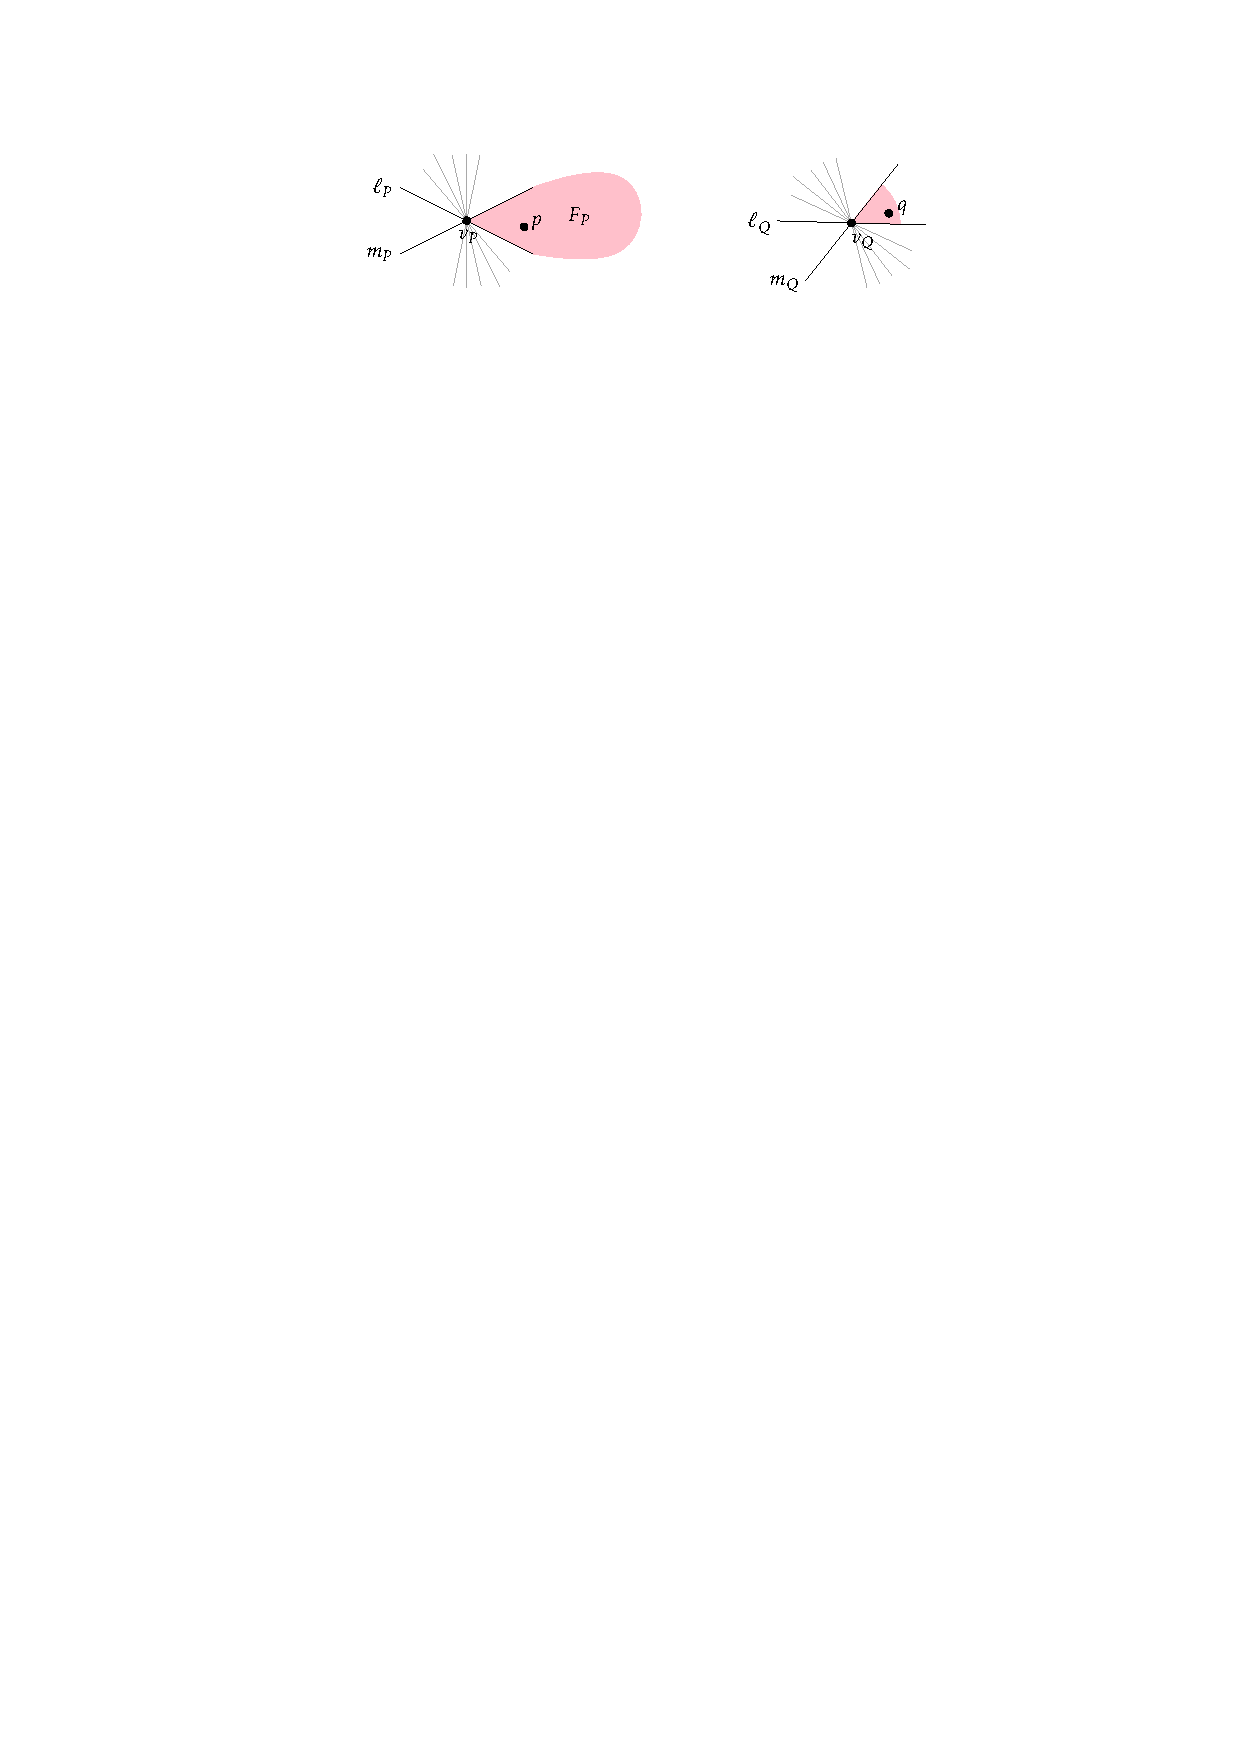
\includegraphics{figs/main-lemma}
      \end{center}
      \caption{The proof of \lemref{main}.}
      \figlabel{main-lemma}
   \end{figure}

   For each $i\in \{1,\ldots,\kappa\}$, let $r_i=|P_i|=|Q_i$ and let
   Let $P_{i}=p_1,\ldots,p_{r_i}$ and $Q_{i}=q_1,\ldots,q_{r_i}$.
   By assumption, we already have that $f(p_i,p_j,p_k)=f(q_i,q_j,q_k)$
   for all $i,j,k\in \{1,\ldots,r_{\kappa-1}\}$.  What remains is to
   find a point $q$ such that $f(p_i,p_j,p) = f(q_i,q_j, q)$ for all
   $i,j\in\{1,\ldots,r_{\kappa-1}\}$.

   The two lines $\ell_Q$ and $m_Q$ correspond (via duality) to two
   points $p_i$ and $p_j$ in $P_{\kappa}$ and the two corresponding
   points $q_i$ and $q_j$ in $Q_{\kappa}$ correpsond to lines $\ell_P$
   and $m_P$ that intersect at some point $v_Q$.

   We now have a point $v_Q$ such that $f(p_i,p_j,v_P)=f(q_i,q_j,v_Q)$
   for all $i\in \{1,\ldots,r_{\kappa-1}\}$.  Furthermore,
   $f(p_i,p_j,v_P)=f(p_i,p_j,p)$ for all $i,j\in
   \{1,\ldots,r_{\kappa-1}\}$ except when $p_i$, $p_j$ and $v_P$ are
   collinear.  To obtain the point $q$ required by the lemma, all we
   have to do is move $v_Q$ within an $\epsilon$-neighbourhood of $v_Q$
   in the right direction in order to obtain $f(p_i,p_j,p)=f(q_i,q_j,q)$
   for those $i,j\in\{1,\ldots,r_{\kappa-1}\}$ such that $p_i$ and
   $p_j$ that are collinear with $p$.  Note that each such pair $(i,j)$
   defines a line containing containing $p_i$, $p_j$ and $v_P$ as well as
   a line containing $q_i$, $q_j$ and $v_Q$.  Furthermore, the ordering
   of these lines around $v_P$ is the same as the (corresponding) lines
   around $v_Q$.  (This last statement is true because full order type
   includes ordering information about collinear points.)  In particular,
   $\ell_Q$ and $m_Q$ occur consecutively in this ordering and a point $q$
   satisfying the conditions of the lemma can be found in the neighbourhood
   of $v_Q$ in the space between one of the (at most 4, though usually 2)
   consecutive ooccurences of $\ell_Q$ and $m_Q$ about $v_Q$.
\end{proof}

\begin{lem}\lemlabel{free}
   Let $G$ be a planar graph.  Then any collinear set in $G$ is a free
   collinear set in $G$.
\end{lem}

\begin{proof}
   Suppose $G$ has a plane drawing with its vertex coordinates at position
   $P=p_1,\ldots,p_n$ so that vertices $p_1,\ldots,p_r$ appear, in order,
   on the $x$-axis.  Therefore, $G$ has a collinear set of size $r$.
   Without loss of generality, we may assume that the $x$-coordinate of
   $p_1$ is greater than 0.

   For a sufficiently small $\epsilon>0$, we can randomly perturb each
   of $p_{r+1},\ldots,p_n$ by a distance of at most $\epsilon$ and
   the drawing will remain a plane drawing. (The supremum such value of
   $\epsilon$ is called the \emph{tolerance} of $G$ \cite{X}.)  After this
   perturbation, the only points on the $x$-axis are $p_1,\ldots,p_r$,
   no two points in $P$ have the same $x$-coordinate and no three
   vertices in the drawing are collinear, unless all three vertices are
   in $p_1,\ldots,p_r$.

   To prove the lemma, we must show that, for any $0<x_1<x_2<\cdots<x_r$
   there exists a plane drawing of $G$ so that $p_i$ is drawn at
   $q_i=(x_i,0)$ for each $i\in\{1,\ldots,r\}$.  We will prove
   something stronger: There exists $q_{r+1},\ldots,q_n$ such that
   the point sequence $q_1,\ldots,q_n$ has the same full order type
   as $p_1,\ldots,p_n$. Since the full order type of a point set
   is sufficient to test if two segments cross and to identify, and
   determine the ordering of, collinear points, the full order type
   contains enough information to determine if a graph drawing is plane.

   We first observe that, for any $k\in\N$,
   $f^{\kappa}_{p_1,\ldots,p_r}=f^{\kappa}_{q_1,\ldots,q_r}$.  Indeed,
   this is easily verified for the case $\kappa=1$ and, for $\kappa>1$,
   the only additional point that appears in $P_\kappa$ and $Q_\kappa$ is
   the dual of the $x$-axis, which is the origin, $(0,0)$.  In particular,
   $f^{\kappa}_{p_1,\ldots,p_r}=f^{\kappa}_{q_1,\ldots,q_r}$ for
   $k=n-r+1$.  Now, by the random perturbation, $p_{r+1}$ satisfies the
   conditions of \lemref{main}, so we can find a point $q_{r+1}$ so that
   $f^{\kappa-1}_{q_1,\ldots,q_{r+1}}=f^{\kappa-1}_{p_1,\ldots,p_{r+1}}$.
   In the same way, for each of $i=2,\ldots,n-r$ we can
   find $q_i$ so that $f^{\kappa-i}_{q_1,\ldots,q_{r+i}} =
   f^{\kappa-i}_{p_1,\ldots,p_{r+i}}$.  In particular, the
   end result is the point sequence $q_1,\ldots,q_n$ such that
   $f^{1}(q_1,\ldots,q_n)=f^{1}(p_1,\ldots,p_n)$, i.e., $q_1,\ldots,q_n$
   has the same full order type as $p_1,\ldots,p_n$.
\end{proof}

\section{Discussion}

Discuss all the consequences of \lemref{free} here\ldots
Basically, any graph class that has a collinear set of size $f(n)$ can 
be untangled while keeping $f(n)$ vertices fixed.  For such graph classes,
every point set of size $f(n)$ is a subset universal for $n$-vertex graphs
in the class.

Our \lemref{free} also holds for other types of graph drawing problems,
as long as the relevant properties of the drawing can be tested using
order types.  This includes, for example, rectillinear $k$-planarity
and geometric thickness $k$ graphs.

To prove this result we created an \emph{ad hoc} refinement of order types
that was sufficient for our particular application and our \lemref{main}
was also just sufficient for our application.  Our \lemref{main} is easily
strengthened to any point $p\in\R^2$, but our definition of $\kappa$
full order types is, for example, not translation invariant for $\kappa
> 1$. This is due to the fact that the point set $P_{\kappa}$ contains
both dual and primal points.  If further applications warrant it, a more
careful definition that separates dual and primal point sets could be
provided that is invariant under affine transformations and for which
\lemref{main} still holds.

\end{document}


